%%%%%%%%%%%%%%%%%%%%%%%%%%
%                          %
% ----- INTRODUCTION ----- %
%                          %
%%%%%%%%%%%%%%%%%%%%%%%%%%

\section{Introduction}

	\subsection{Idée}

		Le but recherché de l'outil est de sensibiliser les utilisateurs aux informations que ceux-ci dévoilent potentiellement en naviguant sur le web. Pour ce faire, nous avons besoin d'amasser des données sur leurs habitudes de navigation afin de les analyser.

		Ces données seront centralisées sur un serveur afin que nous puissions lancer des traitements sur l'ensemble des données plus tard dans le but de tenter de révéler des tendances, habitudes ou corrélations entre les données.

		De plus, nous souhaitons également offrir un service direct à l'utilisateur afin que celui-ci ait un bénéfice à installer l'extension et nous autoriser à accéder à ces données. Nous allons lui montrer via une interface web les données que nous avons pu amasser sur sa navigation depuis l'installation du plug-in, au travers de plusieurs pages et visualisations.

		Nous souhaitons également que les données récupérées ne puissent pas être utilisées pour reconnaître une personne particulière. C'est pourquoi le plug-in ne nécessite aucune connexion avec un compte externe, et ne demande pas information directement divulgatrice d'une identité.

		Nous pouvons ainsi résumer les caractéristiques principales du plug-in en quelques points.

		Le plug-in :
		\begin{itemize}
			\item Récupère les informations de navigation de l'utilisateur
			\item Envoie ces informations de manière anonyme à un serveur centralisé
			\item Propose une visualisation des données récoltées et calculées sur l'utilisateur
		\end{itemize}

	\subsection{Architecture}

		Le projet dans son ensemble requiert le développement d'un minimum de deux parties différentes :

		\begin{itemize}
			\item Une extension pour navigateur afin de récupérer et d'envoyer les données
			\item Un serveur recevant les données des extensions installées
		\end{itemize}

		Une troisième partie s'occupant de l'interface utilisateur est également à prévoir, celle-ci pouvant se situer autant dans l'extension que sur le serveur. La décision est finalement prise d'héberger l'interface utilisateur sur un différent serveur, auquel se connecte l'interface lorsque l'utilisateur souhaite accéder à sa page.

		\begin{figure}[h]
			\centering
			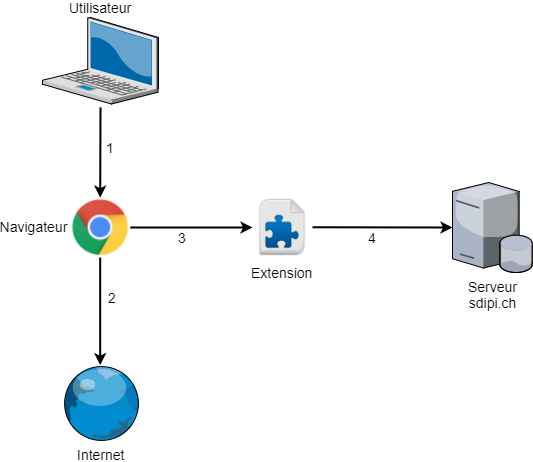
\includegraphics[width=0.8\textwidth]{images/design/intro/architecture}
			\caption{Flux de données de l'extension.}
			\label{d-architecture}
		\end{figure}

		La figure \ref{d-architecture} schématise la récolte de données effectuée par l'etension.
		\begin{enumerate}
			\item L'utilisateur entre une URL dans son navigateur
			\item Le navigateur accède à la ressource concernée
			\item Le navigateur transmet au plug-in les informations concernant la navigation
			\item Le plug-in contacte le serveur SDIPI pour lui transmettre les informations
		\end{enumerate}

	\subsection{Données}\label{d-donnees}

		Les possibilités de récolte de données depuis une extension de navigateur sont extrêmement nombreuses. Nous allons cependant nous concentrer sur l'amassage de données utiles à l'étude, et qui ne représentent pas une menace à l'intimité de l'utilisateur. Nous devons donc nous limiter à un set de données adéquat. 

		Voici les différents types d'informations que nous récoltons, et à quelles fins chaque type d'information est utilisé :

		\subsubsection{Visite d'une URL}
			
			Lorsque l'utilisateur accèds à une nouvelle URL dans son navigateur, qu'il s'agisse d'un clic sur un lien ou d'une entrée dans la barre d'adresse, l'extension enregistre une partie de l'URL accédée ainsi que la date d'accès. Pour des raisons de protection de la vie privée, seule une partie de l'URL est conservée et envoyée au serveur.

			\begin{figure}[h]
				\centering
				$\underbrace{\texttt{https://www.google.ch/search}}_{\text{Partie conservée}}$\texttt{?q=Recherche+test}
				\caption{Exemple d'URL et traitement}
				\label{d-url}
			\end{figure}

			La figure~\ref{d-url} montre que tous les paramètres de la requête ne sont pas conservés. Seuls le protocole (\texttt{http} ou \texttt{https}), le nom de domaine, l'éventuel numéro de port ainsi que le chemin d'accès à la ressource sont conservés. Nous évitons ainsi la possibilité de stocker des informations sensibles comme le nom d'utilisateur, qui peut parfois se trouver dans cette partie de l'URL de certains sites web.

		\subsubsection{Activité sur une page}

			À tout moment, l'utilisateur a probablement plusieurs onglets ou plusieurs fenêtres de navigateur ouvertes. Nous souhaitons nous intéresser à quelle page est actuellement en train d'être parcourure par l'utilisateur. À cette fin, nous détectons les évènements sur la page web : Appui sur une touche, ou clic de souris par exemple. Dès lors qu'il se passe plus de 30 secondes sans aucun évènement de la part de l'utilisateur, nous estimons qu'il ne regarde plus activement la page. Ce temps passé à s'insétresser à chaque page est également envoyé au serveur central toutes les 30 secondes.

		\subsubsection{Requêtes du navigateur}

			Lorsque le navigateur accède à une page web ou à d'autres moments, le navigateur doit charger des ressources qui se trouvent sur un serveur distant. Ce chargement peut prendre place pour afficher par exemple une image, un morceau de la page web elle-même, ou être demandé par un script chargé.

			Pour chaque requête que le navigateur envoie, l'extension mémorise certaines informations : 
			\begin{description}
				\item[Origine] L'extension mémorise l'URL de la page qui demande la ressource. Cette information est traitée de la même manière que décrit à la figure~\ref{d-url}.
				\item[Hôte] Toujours d'une manière identique à la figure~\ref{d-url}, l'extension mémorise également le serveur contacté.
				\item[Taille] L'extension mémorise également la taille de la requête en question, qui correspond à l'addition du contenu envoyé dans le contenu de celle-ci, ainsi que la taille des paramètres (ceux qui ne sont pas retenus par l'extension).
			\end{description}

		\subsubsection{Identificateur}

			Lors de l'installation de l'extension, un nombre aléatoire est généré pour l'installation. Cet identificateur est envoyé envoyé au serveur central en plus de chaque autre information : Elle nous est utile pour assigner chaque donnée de navigation avec un navigateur particulier.

\section{Extension}

	L'extension de navigateur est sans aucun doute la partie la plus simple du projet. Etant donné que nous avons décidé d'héberger l'interface utilisateur sur un serveur différent, l'extension ne va principalement s'occuper que de récupérer les données de l'utilisateur et les transmettre à notre serveur.

	Etant donné qu'une extension de navigateur n'est disponible que pour un type de navigateur à la fois, la question du suport de plusieurs navigateurs s'est posée. D'après le site populaire \texttt{w3schools.com}\cite{browser-stats}, Google Chrome représente plus de 75\% des visites au moins de décembre 2017. Nous décidons donc de ne pas adapter le code de l'extension pour plusieurs types de navigateurs, car nous estimons que le gain en utilisateurs serait insuffisant pour justifier le développement supplémentaire.

	L'extension sera donc développée pour le navigateur Google Chrome, en utilisant l'API JavaScript que celui-ci met à disposition. Les fonctionnalités implémentées sont la récolte et l'envoi des types de données décrites à la section \ref{d-donnees}.

	L'extension proposera également à l'utilisateur d'accéder à l'interface grâce à un lien, ainsi que la possibilité de se "lier" ce navigateur au profil d'un autre navigateur existant, en entrant son ancien identificateur. Ceci permet à un utilisateur de profiter d'un seul profil au travers de plusieurs machines posédant l'extension, par exemple. 

\section{Serveur}

	\subsection{Rôles}

		La partie du serveur est probablement la plus complexe du projet. Le serveur va devoir assurer le fonctionnement de plusieurs tâches clés :

		\begin{itemize}
			\item Récolte et enregistrement des données de l'extension
			\item Traitement des données utilisateurs
			\item API au service de l'interface
		\end{itemize}

	\subsection{Récolte}

		Avant tout traitement, le serveur doit être capable de recevoir et d'enregistrer les données des clients. Etant donné que l'extension est développée en JavaScript, les données seront transmises par HTTP au format JSON pour des raisons de simplicité.

		\subsubsection{Installation du plug-in}

			Au moment où le plug-in est installé, une requête est envoyée au serveur afin de l'avertir qu'un nouvel utilisateur a installé l'extension. Le serveur génère un identifiant, l'envoie à l'extension en réponse et est désormais prêt à recevoir des information de ce nouvel identifiant.

		\subsubsection{Récolte continuelle\label{d-recolte}}

			Afin que le serveur soit capable de supporter une certaine charge d'utilisateurs, il est nécessaire que celui-ci recoive un nombre réduit de requêtes de la part des clients. Pour cette raison, l'extension ne contacte le serveur qu'une seule fois toutes les 30 secondes afin de le tenir informaé des évènement ayant eu lieu.

			Le serveur va donc pouvoir exposer une API simple : L'extension contactera toujours le même endpoint, et chaque requête contiendra la liste des informations concernant les évènements qui se sont passés chez le client.

			Lorsque nous détectons qu'utilisateur visite une URL pour la première fois, le serveur va télécharger le contenu de cette page. Notre serveur ouvre un navigateur virtuel afin de simuler le chargement complet de la page - y compris l'exécution de scripts - et enregistre le contenu final de la page dans la base de données.

			\begin{figure}[!h]
				\centering
				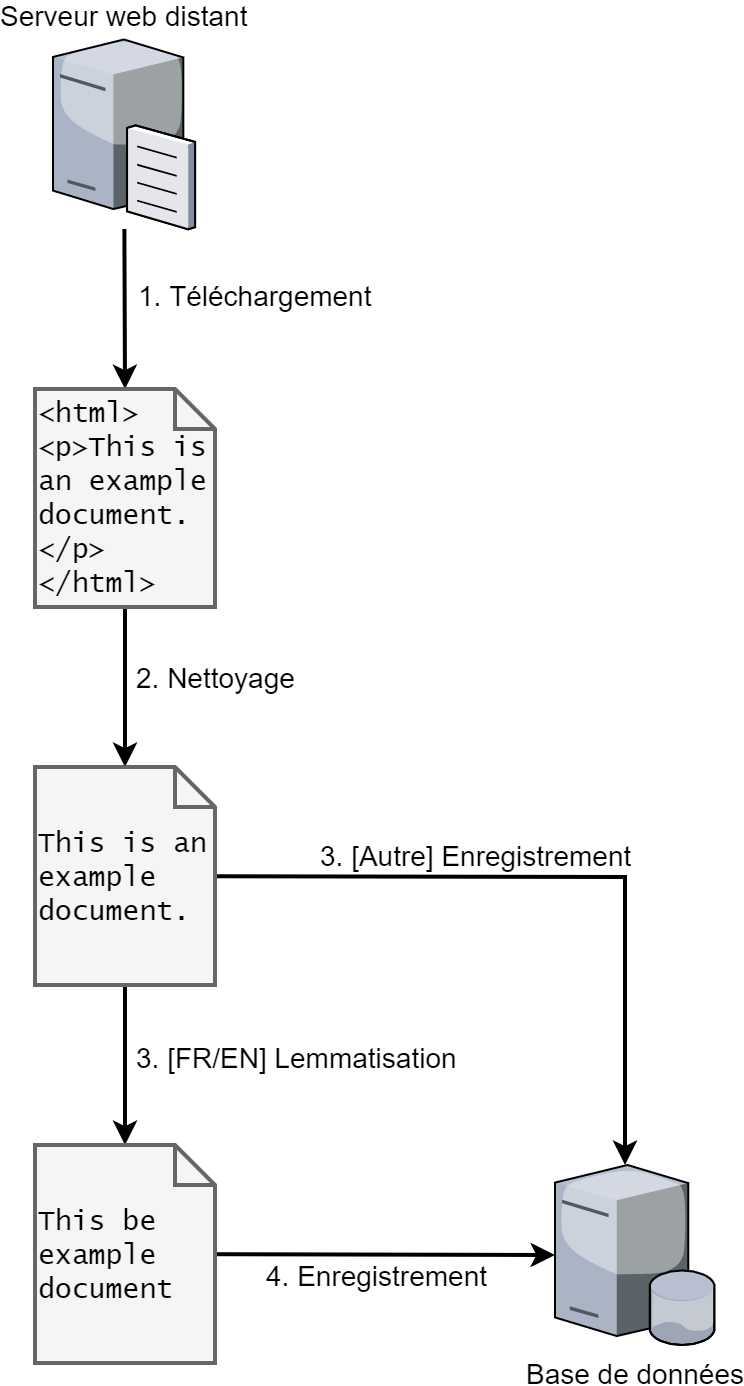
\includegraphics[width=0.5\textwidth]{images/design/data1_big}
				\caption{Téléchargement et enregistrement du contenu d'une page}
				\label{d-download-page}
			\end{figure}

			Une série d'opérations est ensuite effectuée sur le contenu de la page, afin de le rendre utilisable par les prochains algorithmes. La figure~\ref{d-download-page} montre les étapes qui entrent en compte dans le pré-traitement du contenu :

			\begin{description}
				\item[1. Téléchargement] Le serveur lance, dans un navigateur virtual, le téléchargement de la page ainsi que l'exécution des scripts présents sur celle-ci. Une fois la page complètement chargée, on conserve le DOM de la page chargée.
				\item[2. Nettoyage] À partir du HTML de la page, on ne cherche à garder que le texte de celle-ci, sans balise. Un parseur enlève toutes les balises \texttt{<script>} et \texttt{<style>}, puis ne garde que le contenu des éléments restants.
				\item[3. [FR/EN] Lemmatisation] Un détecteur de langue nous renseigne sur la langue du texte. Si celui-ci est en anglais ou en français, nous lemmatisons chaque mot du texte. Ce processus analyse lexicalement les mots présents, et tente de ramener chaque mot à dans une forme plus simple pour le représenter. Par exemple, le temps des verbes est changé en infinitif, et les noms communs perdent leur pluriel. La liste complète des traitements effectuée est en réalité bien plus longue, et propre à la langue du texte.
				\item[3/4. Enregistrement] Si le texte n'est pas dans une langue supportée par la lemmatisation, ou après la lemmatisation du texte anglais ou français, celui-ci est enregistré dans la base de données. Tous les traitements futurs sur le contenu de la page se feront sur cette version-ci.
			\end{description}

	\subsection{Enregistrement}

		Le serveur se charge également de la gestion du stockage des données reçues (et calculées). Une base de données MySQL sera continuellement alimentée par les nouvelles données reçues. La base de données comprendra généralement une table par type de données à enregistrer, ainsi que des tables temporaires dans lesquelles seront placées des informations pré-calculées afin de répondre plus rapidement aux requêtes de l'interface.

	\subsection{Traitement des données}

		Une fois des données enregistrées, celles-ci sont traitées par différentes méthodes en fonction des besoins de l'interface. Voici le traitement que subit chaque type de données. Les traitements décrits ici ne sont pas effectués directement à la réception de données d'un client : Ils sont effectués régulièrement lorsque nécessaire.

		\subsubsection{Quantité de visites}

			Deux mesures sont récoltées sur l'intérêt que peut avoir un utilisateur par rapport à une page web : Le nombre de fois que cette URL a été ouverte, et le temps passé à être actif sur la page en question. Chacune de ces informations est également datée.

		\subsubsection{Contenu des pages}

			Les traitements les plus lourds que nous effectuons prennent en entrée le contenu des pages visitées.

			\begin{figure}[!h]
				\centering
				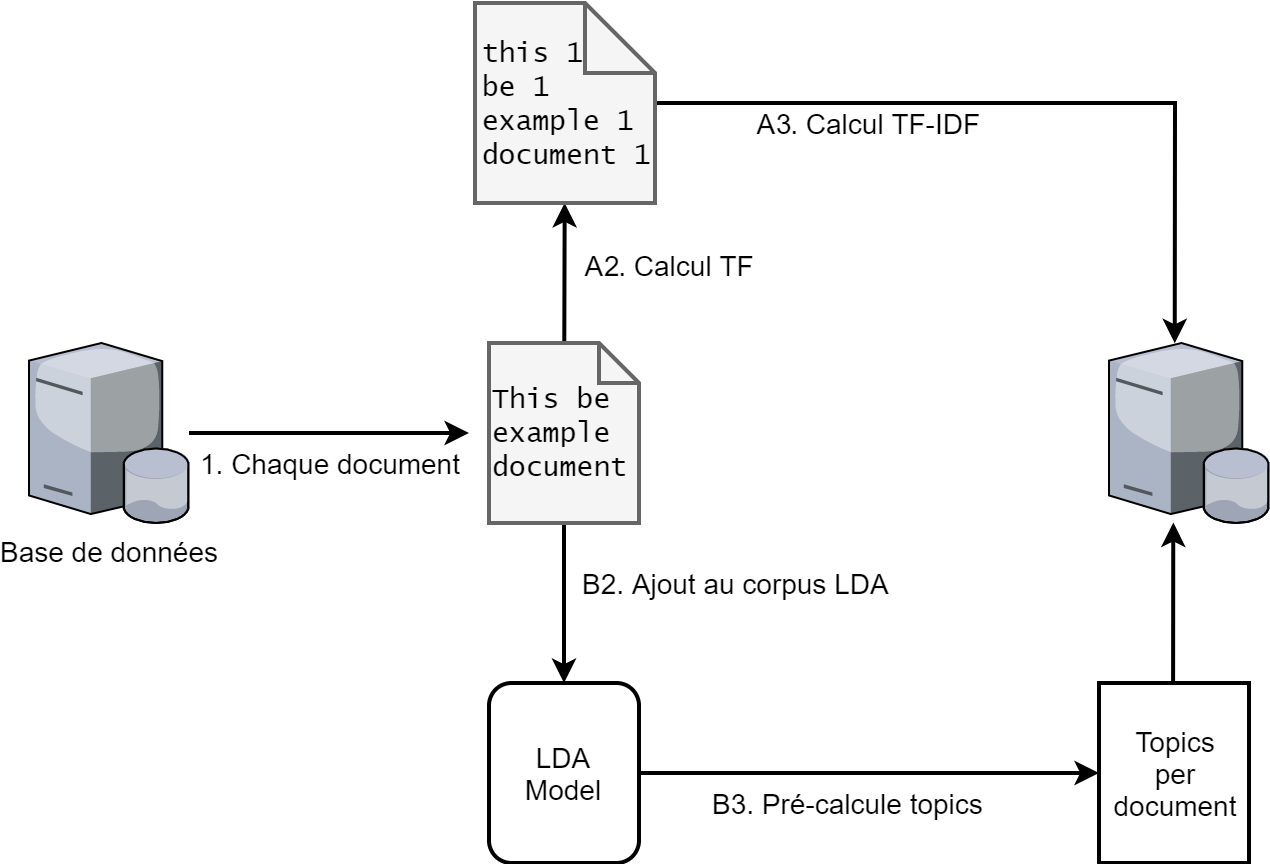
\includegraphics[width=0.8\textwidth]{images/design/traitement_offline}
				\caption{Traitements du contenu des pages}
				\label{d-traitements}
			\end{figure}

			Le contenu de la page est analysé indépendamment par deux algorithmes différents, chacun permettant de révéler un type d'information différent.

			La figure~\ref{d-traitements} montre les deux traitements effectués aux documents de la base de données.

			\begin{description}
				\item[1. Chaque document] le serveur va charger la liste entière des contenus enregistrés des pages web, obtenues comme décrites à la section \ref{d-recolte}.
				\item[A2. Calcul TF] La fréquence de chaque mot du document est calculée, puis enregistrée
				\item[A3. Calcul TF-IDF] Une fois en possession de la fréquence de chaque mot dans chaque document, le poids final TF-IDF normalisé est calculé et enregistré dans la base de données, pour chaque mot à l'intérieur de chaque document.
				\item[B2. Ajout au corpus LDA] Avant de générer un modèle, un traitement semblable à la branche A2 est effectuée pour chaque document. Une fois tous les documents chargés, on lance l'exécution de la génération du modèle LDA.
				\item[B3. Pré-calcule topics] Une le modèle entraîné, processus qui peut facilement durer plusieurs heures, il est enregistré sur le disque. Après quoi, une multitude de requêtes sont effectuées sur le modèle afin de connaître déjà quels sont les topics les plus probables pour chaque page de la base de données. On enregistre les résultats à nouveau dans la base de données. Ce pré-calcul va accélérer considérablement les traitements futurs sur la reconnaissance des topics significatifs pour un utilisateur en fonction des pages web qu'il a visité. 

			\end{description}

			\paragraph{TF-IDF}

				TF-IDF est une méthode permettant de détecter quels sont les mots les plus importants dans un document parmi l'ensemble d'un cropus. La méthode consiste purement en l'analyse de la fréquence de chaque mot dans chaque document, et ne s'occupe absolument pas de la signification des mots.

			\paragraph{LDA}

				LDA est un modèle qui permet de générer un nombre de sujets, thèmes ou topics, en fonction du contenu textuel d'un corpus de documents. Le modèle suppose que chaque document parle de un ou plusieurs topics, et tente de les retrouver en se basant sur la fréquence d'utilisation de ses mots en comparaison avec le reste du corpus de documents. 

		\subsubsection{Requêtes du navigateur}

			Comme mentionné précédemment, quelques informations de chaque requête du navigateur du client sont enregistrées. Ces données n'ont pas besoin d'un traitement particulier.

			Etant donné que nous nous intéressont particulièrement à leur quantité, nous n'allons principalement que les compter. Cependant dû au fait de leur énorme quantité, il nous est nécessaire de pré-calculer certaines sommes avant de les servir à l'interface.

	\subsection{API}

		Le serveur a également le rôle de répondre aux demander de l'interface, et de lui fournir les informations nécessaire pour afficher les données du client. Ces communications se font au travers d'une série de requêtes initiées par le client.

		Une partie des données servies au client sont pré-calculées, comme la liste des topics tirés de LDA ou le poids TF-IDF des mots, et ne sont donc rafraîchies que périodiquement lorsque demandé.

		Le reste des données, comme le nombre d'ouvertures d'une page ou le temps actif passé sur chaque page, est continuellement rafraîchi. Ces données sont donc toujours à jour.

\section{Interface}

	L'interface a connu de nombreuses versions au fur et à mesure du projet. Cependant, le thème et le but commun de ces pages n'a pas changé : Montrer à l'utilisateur les informations qu'il révèle, ainsi que des possibles utilisations de celles-ci. Le design initial des visualisation était très visuel et varié et a progressé vers des pages plus utilitaires.

	L'interface se divise en deux onglets distincs, chacun tentant de représenter une partie des informations. 

	\subsection{Settings}

		La page Settings laisse la possibilité à l'utilisateur de resneigner ces centres d'intérêt en les sélectionneant parmi une liste d'une centaine d'entre-eux. Cette centaine d'intérêts sont ceux que Google utilise pour "classifier" les visiteurs de sites web utilisant Google Analytics, nous estimons donc que ces intérêts font sens. 

	\subsection{Profil}

		\begin{figure}[!h]
			\centering
			\includegraphics[width=0.8\textwidth]{images/design/mockup_profile}
			\caption{Maquette de la page de Profil}
			\label{d-mockup-profile}
		\end{figure}

		La page Profil cherche à montrer le résultat de l'analyse des pages visitées par l'utilisateur, tentant de retrouver et de lui montrer quels sont ses centres d'intérêts. 

		Voici les différentes concepts de visualisations montrées à l'utilisateur :

		\subsubsection{Wordcloud}

			Le wordcloud montre à l'utilisateur la liste des mots qu'il lit le plus fréquemment. Le visualisation est un amassage de mots de différentes tailles, placés d'une manière aléatoire sur un rectangle. Les mots les plus lus ont une taille plus grande afin d'attirer l'attention de l'utilisateur.

			Cette visualisation cherche à donner très rapidement une impression générale des thèmes que l'utilisateur parcourt lors de sa navigation.

		\subsubsection{Topics graph}

			Le "topics graph" cherche à rassembler les mots en thèmes, et monte d'une manière plus synthétique les thèmes estimés que l'utilisateur parcourt fréquamment. À chaque thème est lié un ou plusieurs mots, qui reprèsentent le thème d'une manière générale. Chaque cercle du graphe représente soit un thème, soit un mot.

			Le but de cette visualisation est de montrer que nous pouvons déduire des thèmes et ainsi montrer un traitement plus fin des intérêts de l'utilisateur, que simplement additionner une liste de mots. Dans le marketing, les thèmes découverts pourraient être utilisés pour labelliser les utilisateurs à qui faire apparaître une publicité.

	\subsection{Trackers}

		\begin{figure}[!h]
			\centering
			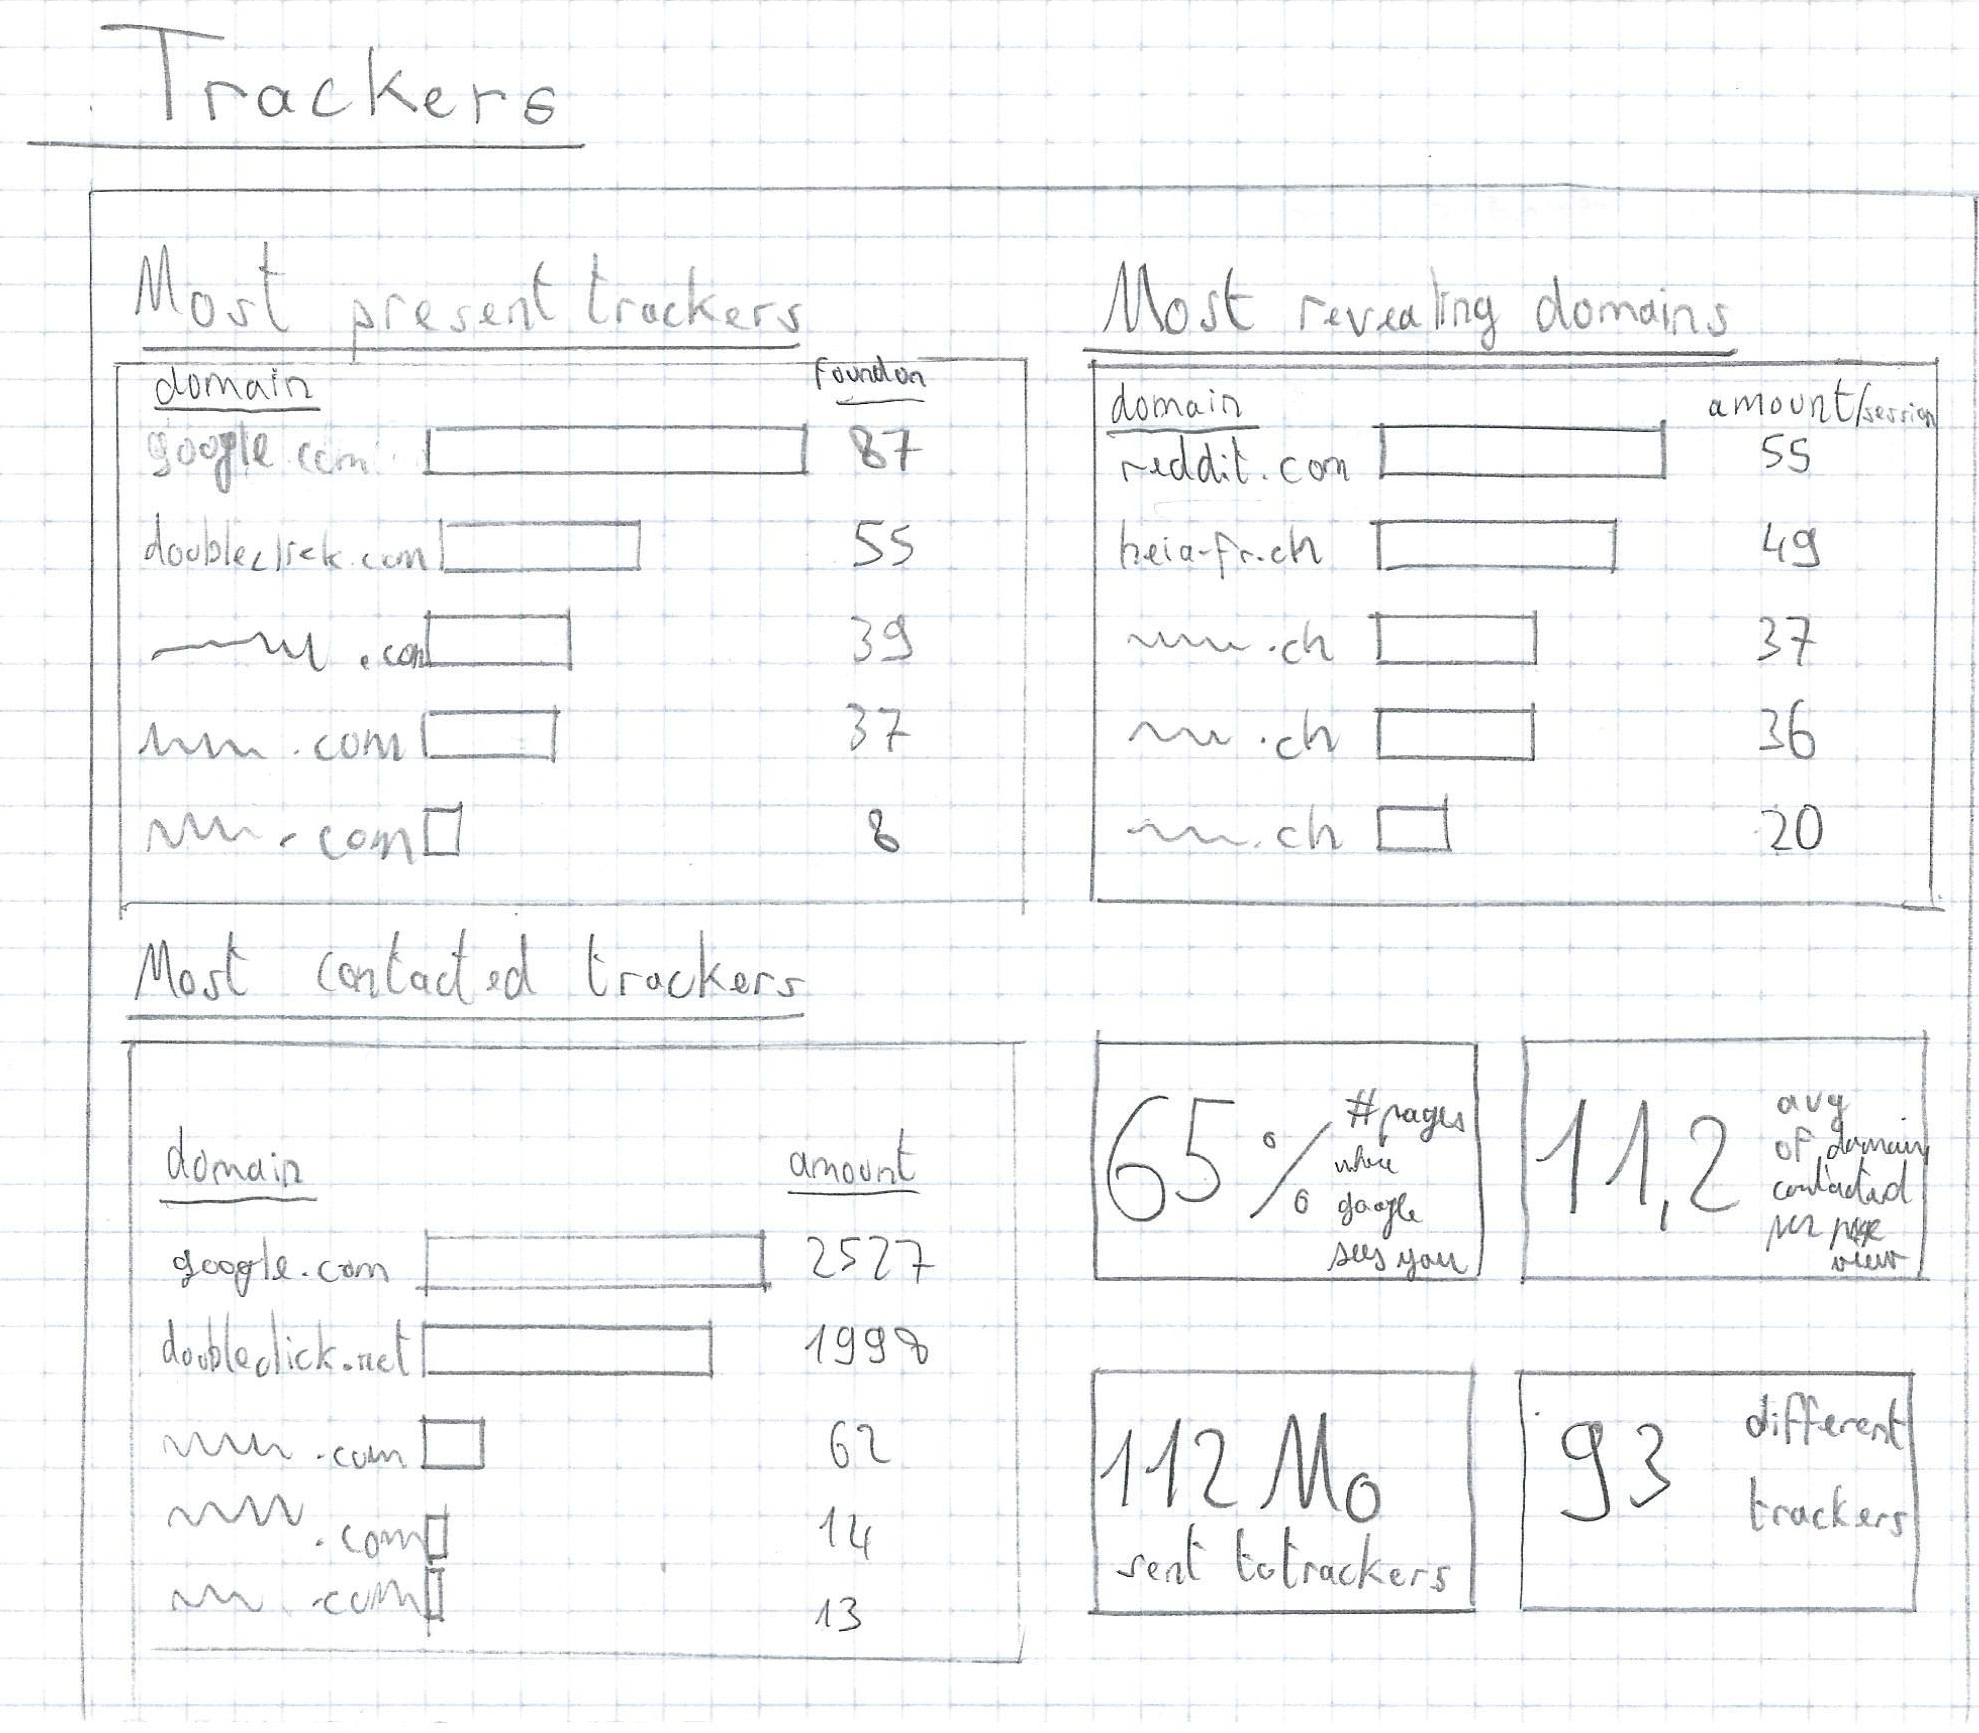
\includegraphics[width=0.8\textwidth]{images/design/mockup_trackers1}
			\caption{Maquette de la page de Trackers}
			\label{d-mockup-trackers1}
		\end{figure}

		\begin{figure}[!h]
			\centering
			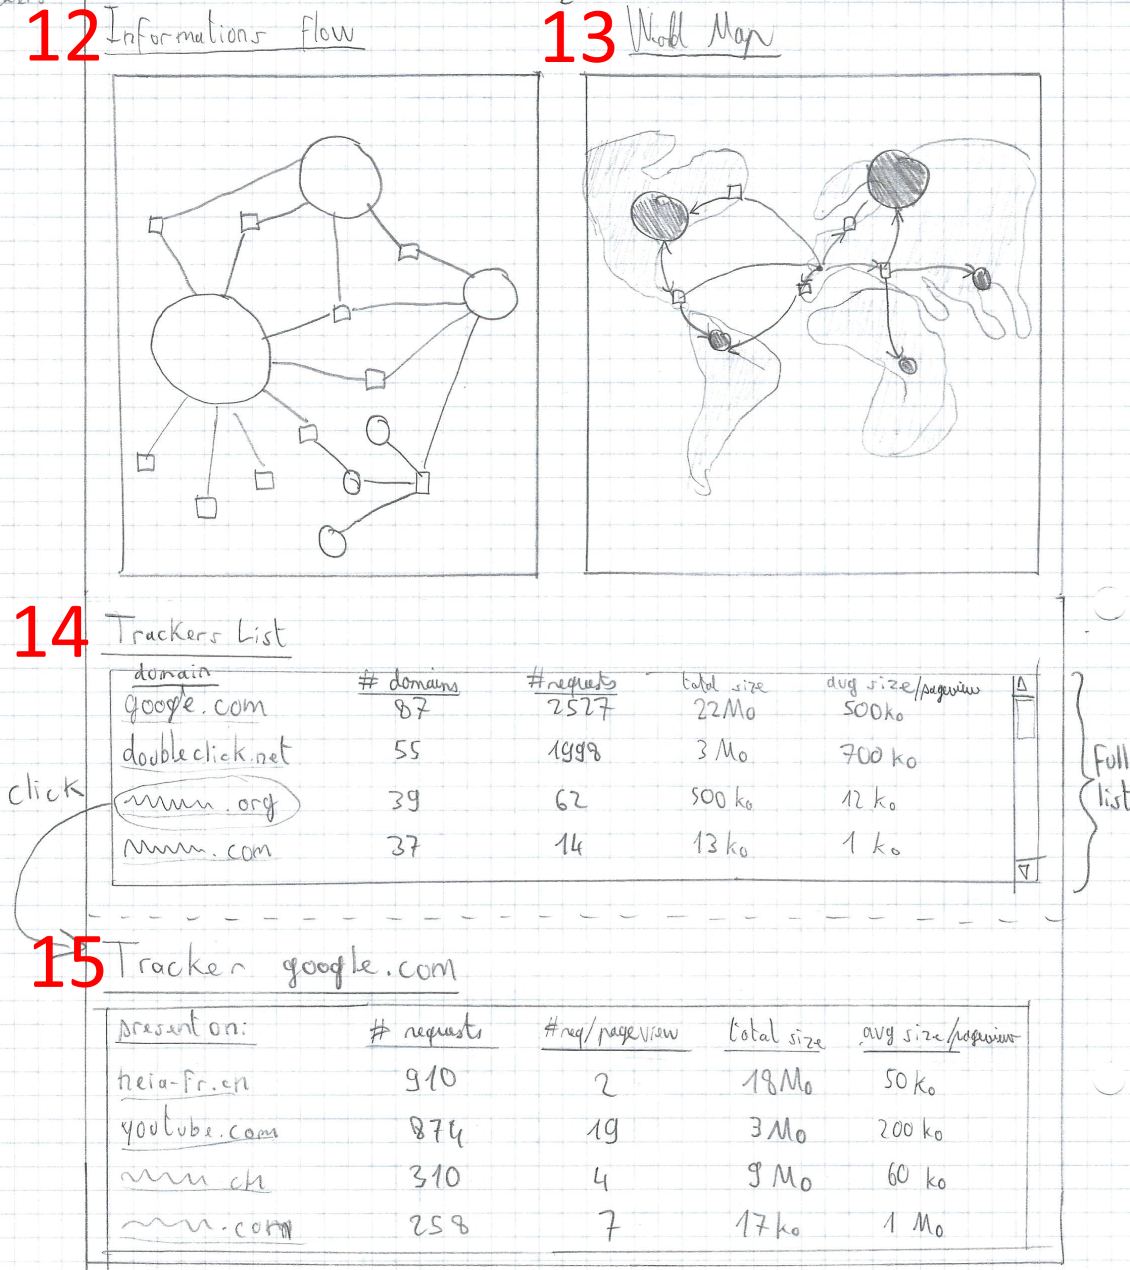
\includegraphics[width=0.8\textwidth]{images/design/mockup_trackers2}
			\caption{Suite de la maquette de la page de Trackers}
			\label{d-mockup-trackers2}
		\end{figure}
